\chapter{Literature Review}

\section{Introduction}
Online two-sided marketplaces and accommodation networks have transformed commerce by reducing transaction costs and pairing supply with demand. However, multi-category platforms combining long-term student tenancy with consumer re-commerce in non-metropolitan hill geographies present distinct algorithmic, architectural, and socio-technical challenges that remain unaddressed by generic platforms. This chapter surveys commercial solutions, analyzes recommendation algorithms, evaluates architectural paradigms, and formalizes practical research gaps in Uttarakhand.

\section{Survey and Critical Evaluation of Existing Systems}
To establish an empirical baseline, we evaluate benchmark platforms across domain focus, transaction models, moderation, and regional adaptability.

\subsection{OLX and Quikr (General Classifieds)}
Horizontal C2C classifieds suffer from lack of domain specialization. In accommodations, OLX fails to capture essential room sharing capacities, floor numbers, meal plans, electricity rules, curfews, or deposit refund policies. Furthermore, absence of pre-publication moderation produces outdated listings and broker spam.

\subsection{Airbnb and Booking.com (Short-Term Hospitality)}
Airbnb provides polished interfaces and calendar bookings, but its financial structure is built for short-term tourism with daily tariffs and 14\%--20\% service fees. Students in Dehradun require semester leasing without recurring percentage charges. Airbnb also lacks student re-commerce integration.

\subsection{Flatmates and Nestaway (Shared Rental Networks)}
Nestaway operates as a managed real estate company with rigid leases, management premiums, and focus limited to Tier-1 metropolises (Bengaluru, Pune, NCR), maintaining zero operational presence in Uttarakhand educational hubs like Dehradun or Roorkee.

\subsection{MagicBricks and 99acres (Commercial Real Estate)}
These platforms monetize through licensed brokers who purchase lead packs. Students seeking affordable ₹5,000/month rooms near Graphic Era Hill University face aggressive broker calls demanding upfront commissions, defeating direct student-to-owner tenancy.

\begin{table}[htbp]
\centering
\caption{Comparative Feature Matrix: StayMart vs. Existing Commercial Platforms}
\label{tab:comparative_matrix}
\footnotesize
\begin{tabularx}{\textwidth}{lccccc}
\toprule
\textbf{Feature Dimension} & \textbf{OLX} & \textbf{Airbnb} & \textbf{MagicBricks} & \textbf{Nestaway} & \textbf{StayMart (Proposed)} \\
\midrule
Primary Focus & Horizontal C2C & Short-Term Stays & Property Sales & Managed Rental & Student Stays + Re-commerce \\
Hyperlocal Granularity & National & Global / Tourist & Metro Agents & Tier-1 Metros & Uttarakhand Corridors \\
Brokerage / Commission & Variable / Spam & 14\%--20\% & Broker Leads & Monthly Margin & \textbf{Zero Brokerage} \\
Room-Level Inventory & No & Whole Property & No & Managed Beds & \textbf{Yes (Single/Double/Dorm)} \\
Re-commerce Integration & Standalone & None & None & None & \textbf{Yes (Unified Marketplace)} \\
Direct In-App Messaging & Basic & Host Only & Lead Form & Agent Support & \textbf{Yes (Real-Time Peer Chat)} \\
ML Recommendation Engine & Static Search & Collaborative & Keyword Filter & Basic Heuristic & \textbf{TF-IDF + Cosine Hybrid} \\
Listing Pre-Moderation & No (Reactive) & Verified & Agent Filtered & Company Audit & \textbf{Yes (Admin Approval Gate)} \\
Realistic Photographic Standard & Low / Stock & High & Stock Render & Managed Shoot & \textbf{Verified (authentic student/host uploads)} \\
\bottomrule
\end{tabularx}
\end{table}

\section{Theoretical Analysis of Recommendation Algorithms}
Recommender systems predict user preference ratings and surface candidate items from catalogues \cite{resnick1997recommender}. We evaluate Collaborative Filtering against Content-Based and Hybrid approaches to justify StayMart's design.

\subsection{Collaborative Filtering (CF) and Its Regional Limitations}
Collaborative Filtering predicts interest based on historical interaction patterns across users \cite{sarwar2001item}. Pearson Correlation evaluates neighborhood similarity:
\begin{equation}
\text{sim}(u, v) = \frac{\sum_{i \in I_{uv}} (r_{u, i} - \bar{r}_u)(r_{v, i} - \bar{r}_v)}{\sqrt{\sum_{i \in I_{uv}} (r_{u, i} - \bar{r}_u)^2} \sqrt{\sum_{i \in I_{uv}} (r_{v, i} - \bar{r}_v)^2}}
\end{equation}
While effective for dense media catalogues \cite{koren2009matrix}, CF fails in regional classifieds due to three obstacles: (1) \textit{Cold-Start Problem}: new room and item listings have zero historical ratings; (2) \textit{Matrix Sparsity}: localized density typically falls below $0.05\%$; (3) \textit{Inventory Exclusivity}: second-hand goods represent single-inventory assets ($N=1$) that vanish upon purchase.

\subsection{Content-Based Filtering (CBF) and Vector Space Modeling}
Content-Based Filtering evaluates item attribute similarity against user preference profiles \cite{lops2011content}. Each listing is synthesized into an attribute document:
\begin{equation}
d = \text{Title} \oplus \text{Description} \oplus \text{Category} \oplus \text{City} \oplus \text{Area} \oplus \text{PriceTier} \oplus \text{Amenities}
\end{equation}
Term Frequency-Inverse Document Frequency (TF-IDF) weights term importance \cite{salton1988term}:
\begin{equation}
\text{TF}(t, d) = \frac{f_{t, d}}{\sum_{t' \in d} f_{t', d}}, \quad \text{IDF}(t, D) = \log\left(\frac{1 + |D|}{1 + |\{d \in D : t \in d\}|}\right) + 1
\end{equation}
\begin{equation}
w_{t, d} = \text{TF}(t, d) \times \text{IDF}(t, D)
\end{equation}
With $L_2$-normalized vectors ($\|\vec{u}\|_2 = 1$), Cosine Similarity simplifies to the dot product, enabling sub-5ms BLAS computations in scikit-learn \cite{pedregosa2011scikit}:
\begin{equation}
\text{CosineSim}(\vec{u}, \vec{v}) = \vec{u}^T \vec{v}
\end{equation}

\subsection{Hybrid Behavioral Re-Ranking Framework}
To combine content cold-start resilience with user engagement signals, StayMart implements a weighted hybrid re-ranking strategy \cite{burke2002hybrid}. Actions $a_k$ are assigned empirical weights: $\text{VIEW} = 1.0$, $\text{SEARCH} = 2.0$, $\text{WISHLIST} = 3.0$, $\text{CONTACT} = 4.0$, $\text{BOOK/ORDER} = 5.0$. The user profile $\vec{p}_u$ incorporates exponential time decay:
\begin{equation}
\vec{p}_u = \sum_{k=1}^m W(a_k) e^{-\lambda \tau_k} \vec{v}_{i_k}
\end{equation}
The composite recommendation score combines cosine similarity, campus proximity, and popularity:
\begin{equation}
S(u, c) = \alpha \cdot \text{CosineSim}(\vec{p}_u, \vec{v}_c) + \beta \cdot \text{LocalityBonus}(u, C_c) + \gamma \cdot \text{PopularityPrior}(c)
\end{equation}
where $\alpha + \beta + \gamma = 1.0$, ensuring recommendations strictly align with the student's geographic corridor.

\section{Architectural Paradigms: Monolithic vs. Distributed Microservices}
In architecting enterprise web applications, the division of responsibilities across compute boundaries is a pivotal design decision \cite{newman2021building, fielding2000architectural}.

\begin{figure}[htbp]
    \centering
    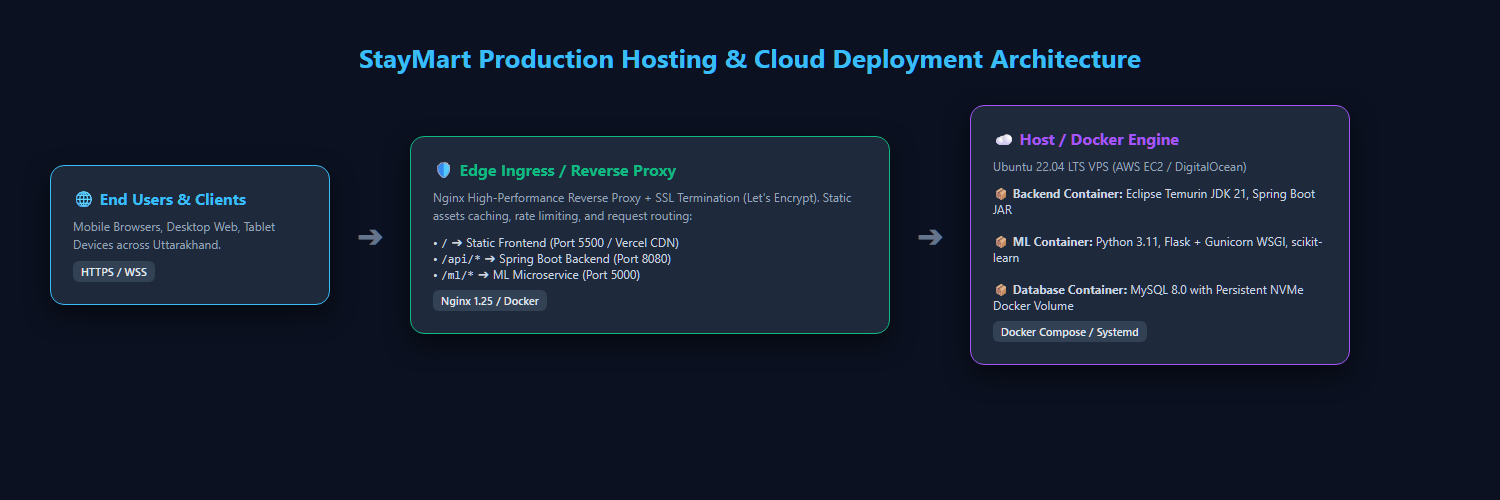
\includegraphics[width=0.92\textwidth]{diagrams/deployment_arch.png}
    \caption{Distributed Microservice Deployment Topology vs. Monolithic Boundaries}
    \label{fig:deployment_topology}
\end{figure}

A monolithic Spring Boot application executes transactional CRUD and intensive ML vector computations within a single JVM. This causes library limitations (Java lacks native scikit-learn parity) and CPU contention during heavy matrix calculations. StayMart adopts a decoupled topology:
\begin{enumerate}
    \item \textbf{Spring Boot 3.3 Core (Port 8080):} Coordinates ACID transactions, JWT authentication, JPA relational entities, and moderation state transitions.
    \item \textbf{Flask ML Microservice (Port 5000):} Operates as an independent service dedicated to TF-IDF transformations, model serialization, and matrix similarity evaluation.
    \item \textbf{Fault-Tolerant Circuit Fallback:} Communication occurs via HTTP REST with 2000ms connect and 3000ms read timeouts. If the ML service is offline, Spring Boot gracefully falls back to database-driven queries matching city and category, eliminating HTTP 500 errors.
\end{enumerate}

\section{Modern Frontend Architectures: Vanilla JS vs. Heavy SPAs}
Modern single-page application (SPA) frameworks (React, Angular) introduce substantial JavaScript payloads (500KB--1.5MB minified) and build fragility, degrading performance on congested campus cellular networks. StayMart intentionally adopts a \textbf{Vanilla HTML5, CSS3, and ES6+ JavaScript} architecture with zero build steps, delivering sub-45 KB payloads, sub-second rendering, and direct static edge deployment on Vercel or CDN nodes.

\section{Identified Practical Gaps and Chapter Summary}
Our systematic review reveals four definitive market gaps: (1) absence of dual-inventory accommodation and re-commerce platforms; (2) lack of Uttarakhand hyperlocal campus granularity; (3) cold-start vulnerability in C2C classifieds; and (4) exploitative brokerage fees. 

In summary, Content-Based TF-IDF vectorization with behavioral re-ranking resolves the sparsity problem, while a decoupled Spring Boot and Flask microservice architecture paired with a lightweight Vanilla JS frontend provides the optimal balance of transactional integrity, ML compute isolation, and mobile performance. The next chapter details system requirements and architectural modeling.
